\documentclass{article}

%
% 引入模板的style文件
%
\usepackage{homework}

\setCJKmainfont{SimSun}[AutoFakeBold] %宋体加粗
\setCJKsansfont{SimHei}[AutoFakeBold] %黑体加粗


\usepackage{minted} %配合minted宏包进行好看的高亮
\usepackage{currfile} %配合minted宏包进行好看的高亮
\usepackage{caption} %配合minted宏包进行好看的高亮
\usepackage{tcolorbox} %配合minted宏包进行好看的高亮
\usepackage{xcolor} %配合minted宏包进行好看的高亮
\tcbuselibrary{skins} %配合minted宏包进行好看的高亮
\tcbuselibrary{minted} %配合minted宏包进行好看的高亮
\usemintedstyle{paraiso-dark} %配合minted宏包进行好看的高亮



%
% 封面
%

\title{
	
\includegraphics[width=0.5\textwidth]{images/title/ucas_logo 1.pdf}\\
    \vspace{1in}
    \textmd{\textbf{\hmwkClass}}\\
    \textmd{\textbf{\hmwkTitle}}\\
    \normalsize\vspace{0.1in}\large{\hmwkCompleteTime }\\
    \vspace{0.1in}\large{\textit{\hmwkClassInstructor\ }}\\
    \vspace{1in}
	
\includegraphics[width=0.25\textwidth]{images/title/Cyber.jpg}\\
	\vspace{1in}
}


\author{
	\hmwkAuthorName \\ 
	\hmwkAuthorStuID \\
	\hmwkAuthorInst \\
	\hmwkAuthorzhuanye \\
	\hmwkAuthorfangxiang
	}
\date{}

\renewcommand{\part}[1]{\textbf{\large Part \Alph{partCounter}}\stepcounter{partCounter}\\}


%
% 正文部分
%
\begin{document}


\maketitle


%\include{chapters/ch01}
%\include{chapters/ch02}
%\include{chapters/ch03}
%\include{chapters/ch04}
%\include{chapters/ch05}


\pagebreak

\begin{homeworkProblem}
	设以下模式类别具有正态概率密度函数:
	$$\omega _1: \left\{ \left( 0,0 \right) ^{\mathrm{T}},\left( 2,0 \right) ^{\mathrm{T}},\left( 2,2 \right) ^{\mathrm{T}},\left( 0,2 \right) ^{\mathrm{T}} \right\} ,\quad \omega _2: \left\{ \left( 4,4 \right) ^{\mathrm{T}},\left( 6,4 \right) ^{\mathrm{T}},\left( 6,6 \right) ^{\mathrm{T}},\left( 4,6 \right) ^{\mathrm{T}} \right\} 
	$$
	(1). 设$P(\omega_1)=P(\omega_2)=1/2$, 求这两类模式之间的贝叶斯判别界面的方程式;\quad 
	(2). 绘出判别界面.
	\\

	\solution
	\\

	\textbf{(1).} 易知正态分布模式的贝叶斯判别函数为
	\begin{align}
		d_i\left( \boldsymbol{x} \right) =\ln P\left( \omega _i \right) -\frac{1}{2}\ln \left| \boldsymbol{C}_i \right|-\frac{1}{2}\left( \boldsymbol{x}-\boldsymbol{m}_i \right) ^{\mathrm{T}}\boldsymbol{C}_{i}^{-1}\left( \boldsymbol{x}-\boldsymbol{m}_i \right) , i=1,2
	\end{align}
	
	模式的均值向量$\boldsymbol{m}_i$和协方差矩阵$\boldsymbol{C}_i$可用下式估计:
	\begin{align}
		\widehat{\boldsymbol{m}}_i=\frac{1}{N_i}\sum_{j=1}^{N_i}{\boldsymbol{x}^{\left( j \right)}},\quad \widehat{\boldsymbol{C}}_i=\frac{1}{N_i}\sum_{j=1}^{N_i}{\left( \boldsymbol{x}^{\left( j \right)}-\widehat{\boldsymbol{m}}_i \right) \left( \boldsymbol{x}^{\left( j \right)}-\widehat{\boldsymbol{m}}_i \right) ^{\mathrm{T}}}, i=1,2
	\end{align}

	其中$N_i$为类别$\omega_i$中的模式的样本数量, 于是由上式计算出:
	\begin{align}
		\widehat{\boldsymbol{m}}_1=\left( \begin{array}{c}
			1\\
			1\\
		\end{array} \right) , \widehat{\boldsymbol{m}}_2=\left( \begin{array}{c}
			5\\
			5\\
		\end{array} \right) , \widehat{\boldsymbol{C}}_1=\left( \begin{matrix}
			1&		0\\
			0&		1\\
		\end{matrix} \right) , \widehat{\boldsymbol{C}}_2=\left( \begin{matrix}
			1&		0\\
			0&		1\\
		\end{matrix} \right) 
	\end{align}
	
	显然$\widehat{\boldsymbol{C}}_1=\widehat{\boldsymbol{C}}_2=\boldsymbol{C}$, 于是有:
	\begin{align}
		d_i\left( \boldsymbol{x} \right) &=\ln P\left( \omega _i \right) -\frac{1}{2}\ln \left| \boldsymbol{C} \right|-\frac{1}{2}\left( \boldsymbol{x}^{\mathrm{T}}\boldsymbol{C}^{-1}\boldsymbol{x}-\underset{1\times 1\text{的数}}{\underbrace{\boldsymbol{x}^{\mathrm{T}}\boldsymbol{C}^{-1}\boldsymbol{m}_i}}-\underset{1\times 1\text{的数}}{\underbrace{{\boldsymbol{m}_i}^{\mathrm{T}}\boldsymbol{C}^{-1}\boldsymbol{x}}}+{\boldsymbol{m}_i}^{\mathrm{T}}\boldsymbol{C}^{-1}\boldsymbol{m}_i \right) \notag
		\\
		&=\ln P\left( \omega _i \right) -\frac{1}{2}\ln \left| \boldsymbol{C} \right|-\frac{1}{2}\left( \boldsymbol{x}^{\mathrm{T}}\boldsymbol{C}^{-1}\boldsymbol{x}-\left( \boldsymbol{x}^{\mathrm{T}}\boldsymbol{C}^{-1}\boldsymbol{m}_i \right) ^{\mathrm{T}}-{\boldsymbol{m}_i}^{\mathrm{T}}\boldsymbol{C}^{-1}\boldsymbol{x}+{\boldsymbol{m}_i}^{\mathrm{T}}\boldsymbol{C}^{-1}\boldsymbol{m}_i \right) \notag
		\\
		&=\ln P\left( \omega _i \right) -\frac{1}{2}\ln \left| \boldsymbol{C} \right|-\left( \frac{1}{2}\boldsymbol{x}^{\mathrm{T}}\boldsymbol{C}^{-1}\boldsymbol{x}-{\boldsymbol{m}_i}^{\mathrm{T}}\boldsymbol{C}^{-1}\boldsymbol{x}+\frac{1}{2}{\boldsymbol{m}_i}^{\mathrm{T}}\boldsymbol{C}^{-1}\boldsymbol{m}_i \right) , i=1,2 \notag
	\end{align}

	由于$P(\omega_1)=P(\omega_2)$, 从而有贝叶斯判别界面的方程式:
	\begin{align}
		d_1\left( \boldsymbol{x} \right) -d_2\left( \boldsymbol{x} \right) &=\left( \boldsymbol{m}_1-\boldsymbol{m}_2 \right) ^{\mathrm{T}}\boldsymbol{C}^{-1}\boldsymbol{x}-\frac{1}{2}{\boldsymbol{m}_1}^{\mathrm{T}}\boldsymbol{C}^{-1}\boldsymbol{m}_1+\frac{1}{2}{\boldsymbol{m}_2}^{\mathrm{T}}\boldsymbol{C}^{-1}\boldsymbol{m}_2=-4x_1-4x_2+24=0
	\end{align}

	\textbf{(2).} 判别界面方程可化简为$x_1+x_2=6$, 于是判别界面如下图所示:
	\begin{figure}[H]  % 这里记得用[H]
		\centering
		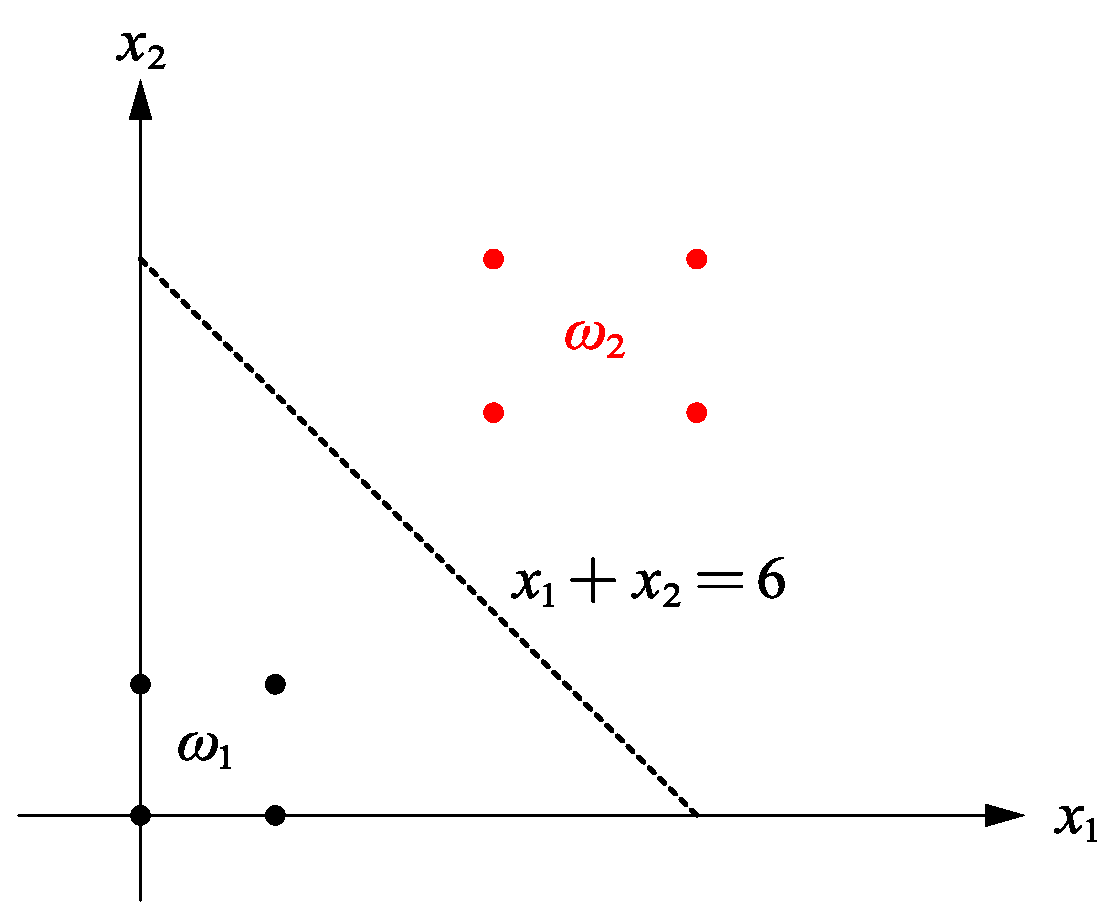
\includegraphics[width=0.4\textwidth]{images/title/判别界面.pdf}
		\caption{判别界面}
		\label{fig:判别界面}
	\end{figure}
\end{homeworkProblem}

\pagebreak

\begin{homeworkProblem}
	编写两类正态分布模式的贝叶斯分类程序(可选例题或上述作业题为分类模式).
	
	正态分布模式的贝叶斯判别$\mathtt{bayes\,\,discrimination()}$函数编码如下(其中$a$是用来控制例题数据或作业题数据的变量, $a=1$表示以作业题数据作为输入, $a=0$表示例题数据作为输入):
\begin{tcblisting}{listing engine=minted,boxrule=0.1mm,
	colback=blue!5!white,colframe=blue!75!black,
	listing only,left=5mm,enhanced,sharp corners=all,
	overlay={\begin{tcbclipinterior}\fill[red!20!blue!20!white] (frame.south west)
	rectangle ([xshift=5mm]frame.north west);\end{tcbclipinterior}},
	minted language=python,
	minted style=tango,
	minted options={fontsize=\normalsize,breaklines,autogobble,linenos,numbersep=3mm}}
import numpy as np
import sympy as sp

def bayes_discrimination(a, pw1, pw2, X_1, X_2):
    N_1 = (X_1[0].shape)[0]  #获取样本个数
    N_2 = (X_2[0].shape)[0]  #获取样本个数

    m_1 = np.mean(X_1,axis=1)  #计算均值向量m_1
    m_1 = np.matrix(m_1).T
    m_2 = np.mean(X_2,axis=1)  #计算均值向量m_2
    m_2 = np.matrix(m_2).T

    Cov_1 = np.cov(X_1)  #计算协差阵Cov_1
    C_1 = Cov_1*(N_1-1)/(N_1)  #修正协差阵为C_1
    C_1 = np.matrix(C_1)
    Cov_2 = np.cov(X_2)  #计算协差阵Cov_2
    C_2 = Cov_2*(N_2-1)/(N_2)  #修正协差阵为C_2
    C_2 = np.matrix(C_2)

    det_C1 = np.linalg.det(C_1) #计算协差阵的行列式
    det_C2 = np.linalg.det(C_2) #计算协差阵的行列式

    ###求取贝叶斯判别函数d_i(x)###
    if(a == 0):
        x = np.matrix([sp.Symbol('x_1'), sp.Symbol('x_2'), sp.Symbol('x_3')]).T
    elif(a == 1):
        x = np.matrix([sp.Symbol('x_1'), sp.Symbol('x_2')]).T
    D_1 = np.log(pw1) - 0.5 * np.log(det_C1) - 1/2 * (x - m_1).T.dot(C_1.I).dot(x - m_1)  #判别函数d_1(x)
    D_2 = np.log(pw2) - 0.5 * np.log(det_C2) - 1/2 * (x - m_2).T.dot(C_2.I).dot(x - m_2)  #判别函数d_2(x)
    D = np.log(pw1) - np.log(pw2) + (m_1 - m_2).T.dot(C_1.I).dot(x) + \
        1/2 * m_2.T.dot(C_1.I).dot(m_2) - 1/2 * m_1.T.dot(C_1.I).dot(m_1)  #特殊情形下简化后的判别界面方程表达式
    print('d_1(x)=', sp.simplify(D_1), sep = '\n')  #打印判别函数d_1(x)
    print('d_2(x)=',sp.simplify(D_2), sep = '\n')  #打印判别函数d_2(x)
    print('d_1(x)-d_2(x)=',sp.simplify(D_1-D_2), sep = '\n')  #直接相减得到的通用判别界面方程
    print('D=',sp.simplify(D))  #特殊情形下判别界面方程的简化表达式
    return
\end{tcblisting}

主函数编码如下: 

\begin{tcblisting}{listing engine=minted,boxrule=0.1mm,
	colback=blue!5!white,colframe=blue!75!black,
	listing only,left=5mm,enhanced,sharp corners=all,
	overlay={\begin{tcbclipinterior}\fill[red!20!blue!20!white] (frame.south west)
	rectangle ([xshift=5mm]frame.north west);\end{tcbclipinterior}},
	minted language=python,
	minted style=tango,
	minted options={fontsize=\normalsize,breaklines,autogobble,linenos,numbersep=3mm}}
if __name__ == "__main__":
    a = input('例题请输入0, 作业题请输入1: ')
    a = int(a)
if(a == 0):
    ##### 以下是例题的输入数据 #####
    pw1 = 0.5  ##这里输入先验概率pw1
    pw2 = 0.5  ##这里输入先验概率pw2
    X_1 = np.array([[1, 0, 1, 1], [0, 0, 1, 0], [1, 0, 0, 0]]) #输入样本矩阵X_1
    X_2 = np.array([[0, 0, 0, 1], [0, 1, 1, 1], [1, 1, 0, 1]]) #输入样本矩阵X_2
    ##### 以上是例题的输入数据 #####
    bayes_discrimination(a, pw1, pw2, X_1, X_2) ##输出判别函数和判别界面方程
elif(a == 1):
    ##### 以下是作业题的输入数据 #####
    pw1 = 0.5  #这里输入先验概率pw1
    pw2 = 0.5  #这里输入先验概率pw2
    X_1 = np.array([[0, 2, 2, 0],[0, 0, 2, 2]]) #输入样本矩阵X_1
    X_2 = np.array([[4, 6, 6, 4],[4, 4, 6, 6]]) #输入样本矩阵X_2
    ##### 以上是作业题的输入数据 #####
    bayes_discrimination(a, pw1, pw2, X_1, X_2) ##输出判别函数和判别界面方程
\end{tcblisting}


上述程序已保存为$\mathtt{chap1.py}$脚本, $\mathtt{conda}$的$\mathtt{base}$环境里装了$\mathtt{numpy}$和$\mathtt{sympy}$库之后, 在终端里执行命令: $\mathtt{python\,\,chap1.py}$, 即可输出作业题的判别函数$d_1\left( \boldsymbol{x} \right),d_2\left( \boldsymbol{x} \right)$分别为
\begin{align}
	d_1(\boldsymbol{x})&=d_1\left( x_1,x_2 \right) =-0.5x_{1}^{2}+1.0x_1-0.5x_{2}^{2}+1.0x_2-1.6931,\\
	d_1(\boldsymbol{x})&=d_2\left( x_1,x_2 \right) =-0.5x_{1}^{2}+5.0x_1-0.5x_{2}^{2}+5.0x_2-25.6931
\end{align}

相应的界面判别方程为
\begin{align}
	D\left( \boldsymbol{x} \right) =D\left( x_1,x_2 \right) =d_1\left( \boldsymbol{x} \right) -d_2\left( \boldsymbol{x} \right) =-4.0x_1-4.0x_2+24.0=0
\end{align}

也得到例题的判别函数$d_1\left( \boldsymbol{x} \right),d_2\left( \boldsymbol{x} \right)$分别为
\begin{align}
	d_1\left( \boldsymbol{x} \right) &=-4.0x_{1}^{2}+4.0x_1x_2+4.0x_1x_3+4.0x_1-4.0x_{2}^{2}-4.0x_2x_3-4.0x_{3}^{2}+0.5794
\end{align}
\begin{align}
	d_2\left( \boldsymbol{x} \right) &=-4.0x_{1}^{2}+4.0x_1x_2+4.0x_1x_3-4.0x_1-4.0x_{2}^{2}-4.0x_2x_3+8.0x_2-4.0x_{3}^{2}+8.0x_3-3.4206
\end{align}

相应的界面判别方程为
\begin{align}
	D\left( \boldsymbol{x} \right) =D\left( x_1,x_2,x_3 \right) =d_1\left( \boldsymbol{x} \right) -d_2\left( \boldsymbol{x} \right) =8.0x_1-8.0x_2-8.0x_3+4.0=0
\end{align}

\end{homeworkProblem}

\pagebreak

\begin{homeworkProblem}
	结合生活中的例子, 出一道用贝叶斯判别及贝叶斯最小风险判别求解的题目.

	\textbf{(1).} 假设某地区居民的新冠感染率为0.005, 居民的状态只有感染$(\omega_1)$和非感染$(\omega_2)$两种. 现在\textbf{国家查得}某核酸机构的数据得知假阳性的比例为0.05, 假阴性的比例为0.01. 若已知某个人的核酸检测结果呈阳性, 则他最可能处于什么状态?
	\\
		
	\solution
	\\

	根据题意易知$P\left( \omega _1 \right) =0.005,P\left( \omega _2 \right) =0.995,p\left( x=\text{阳}|\omega _2 \right) =0.05,p\left( x=\text{阴}|\omega _1 \right) =0.01$.
	根据贝叶斯公式有如下:
	\begin{align}
		P\left( \omega _1|x=\text{阳} \right) &=\frac{P\left( \omega _1 \right) p\left( x=\text{阳}|\omega _1 \right)}{\displaystyle \sum_{i=1}^2{P\left( \omega _i \right) p\left( x=\text{阳}|\omega _i \right)}}=\frac{0.005\times 0.99}{0.005\times 0.99+0.995\times 0.05}=0.0904936 \notag
		\\
		P\left( \omega _2|x=\text{阳} \right) &=\frac{P\left( \omega _2 \right) p\left( x=\text{阳}|\omega _2 \right)}{\displaystyle \sum_{i=1}^2{P\left( \omega _i \right) p\left( x=\text{阳}|\omega _i \right)}}=\frac{0.05\times 0.995}{0.005\times 0.99+0.995\times 0.05}=0.909506 \notag
	\end{align}
	由于$P\left( \omega _1|x=\text{阳} \right) <P\left( \omega _2|x=\text{阳} \right) \therefore x\in \omega _2$, 因此可以得知该核酸机构是吃干饭的. 
	
	\textbf{(2).} 国家为了防止某些检测机构投机倒把、指阳为阴、指阴为阳, 现需要对核酸机构进行相应的罚款来予以匡正. 因此不妨设出一个假阳性的国家罚款为$L_{21}$(元)、出一个\textbf{假阴性}\footnote{请读者仔细思考为何假阴性的影响比较恶劣(不论机构是有意的还是无意的), 这在罚款数中也可体现出来.}的国家罚款为$L_{12}$(元). 现在国家询问某UCAS学子: 应当怎样指定罚款$L_{21}$和$L_{12}$来确保核酸机构很难弄虚作假且精准检测.
	\\
		
	\solution
	\\

	先计算当拿到阳性报告时的各类平均风险:
	\begin{align}
		r_1\left( x=\text{阳} \right) &=\underset{L_{11}=0\left( \text{表示不失分} \right)}{\underbrace{L_{11}p\left( x=\text{阳}|\omega _1 \right) P\left( \omega _1 \right) }}+L_{21}p\left( x=\text{阳}|\omega _2 \right) P\left( \omega _2 \right) =L_{21}\times 0.05\times 0.995 \notag
		\\
		r_2\left( x=\text{阳} \right) &=L_{12}p\left( x=\text{阳}|\omega _1 \right) P\left( \omega _1 \right) +\underset{L_{22}=0\left( \text{表示不失分} \right)}{\underbrace{L_{22}p\left( x=\text{阳}|\omega _2 \right) P\left( \omega _2 \right) }}=L_{12}\times 0.99\times 0.005 \notag
	\end{align}
	再计算当拿到阴性报告时的各类平均风险:
	\begin{align}
		r_1\left( x=\text{阴} \right) &=\underset{L_{11}=0\left( \text{表示不失分} \right)}{\underbrace{L_{11}p\left( x=\text{阴}|\omega _1 \right) P\left( \omega _1 \right) }}+L_{21}p\left( x=\text{阴}|\omega _2 \right) P\left( \omega _2 \right) =L_{21}\times 0.95\times 0.995 \notag
		\\
		r_2\left( x=\text{阴} \right) &=L_{12}p\left( x=\text{阴}|\omega _1 \right) P\left( \omega _1 \right) +\underset{L_{22}=0\left( \text{表示不失分} \right)}{\underbrace{L_{22}p\left( x=\text{阴}|\omega _2 \right) P\left( \omega _2 \right) }}=L_{12}\times 0.01\times 0.005 \notag
	\end{align}
	现在需要使得拿到阳性样本时判别为$\omega_1$和拿到阴性样本时判别为$\omega_2$的平均风险都最小, 即$$L_{12}\times 0.01\times 0.005<L_{21}\times 0.95\times 0.995,\,\,L_{21}\times 0.05\times 0.995<L_{12}\times 0.99\times 0.005$$
	解得不等式为$0<\frac{L_{12}}{18905}<L_{21}<\frac{99L_{12}}{995}$, 于是可选罚款数为$L_{12}=18905,L_{21}=1881$来确保核酸机构不能投机倒把的发国难财且精准检测.
	\newpage
	
\end{homeworkProblem}

\pagebreak







% 引用文献
%\bibliographystyle{unsrt}  % unsrt:根据引用顺序编号
%\bibliography{refs}


\end{document}
